\subsection{Data MC comparison plots for $M_{T}(HH)$ variable used in the fit and for a BDT distribution. Low and high mass regions are shown for both electron and muon channels}

\begin{figure}[tbp]
  \begin{center}
    \includegraphics[width=0.31\textwidth]{figures/mm_300_july20/hhMt_mm_SR_FullPostfit_plot_july20.png}
    \includegraphics[width=0.31\textwidth]{figures/mm_300_july20/hhMt_mm_CRDY_FullPostfit_plot_july20.png}
    \includegraphics[width=0.31\textwidth]{figures/mm_300_july20/hhMt_mm_CRTT_FullPostfit_plot_july20.png}\\
    \includegraphics[width=0.31\textwidth]{figures/mm_300_july20/bdt_response_mm_SR_FullPostfit_plot_july20.png}
    \includegraphics[width=0.31\textwidth]{figures/mm_300_july20/bdt_response_mm_CRDY_FullPostfit_plot_july20.png}
    \includegraphics[width=0.31\textwidth]{figures/mm_300_july20/bdt_response_mm_CRTT_FullPostfit_plot_july20.png}\\
    \caption{Comparison of data and MC samples. 300 GeV, mm channel, Full Postfit plots. Top: hhMt, bottom: BDT distributions. From left to right: SR, CRDY, CRTT.}
    \label{fig:MCcomparison_mm_300}
  %\end{center}
%\end{figure}


%\begin{figure}[tbp]
 % \begin{center}
    \includegraphics[width=0.31\textwidth]{figures/ee_300_july20/hhMt_ee_SR_FullPostfit_plot_july20.png}
    \includegraphics[width=0.31\textwidth]{figures/ee_300_july20/hhMt_ee_CRDY_FullPostfit_plot_july20.png}
    \includegraphics[width=0.31\textwidth]{figures/ee_300_july20/hhMt_ee_CRTT_FullPostfit_plot_july20.png}\\
    \includegraphics[width=0.31\textwidth]{figures/ee_300_july20/bdt_response_ee_SR_FullPostfit_plot_july20.png}
    \includegraphics[width=0.31\textwidth]{figures/ee_300_july20/bdt_response_ee_CRDY_FullPostfit_plot_july20.png}
    \includegraphics[width=0.31\textwidth]{figures/ee_300_july20/bdt_response_ee_CRTT_FullPostfit_plot_july20.png}\\
    \caption{Comparison of data and MC samples. 300 GeV, ee channel, Full Postfit plots. Top: hhMt, bottom: BDT distributions. From left to right: SR, CRDY, CRTT.}
    \label{fig:MCcomparison_ee_300}
  \end{center}
\end{figure}




\begin{figure}[tbp]
  \begin{center}
    \includegraphics[width=0.31\textwidth]{figures/mm_900_july20/hhMt_mm_SR_FullPostfit_plot_july20.png}
    \includegraphics[width=0.31\textwidth]{figures/mm_900_july20/hhMt_mm_CRDY_FullPostfit_plot_july20.png}
    \includegraphics[width=0.31\textwidth]{figures/mm_900_july20/hhMt_mm_CRTT_FullPostfit_plot_july20.png}\\
    \includegraphics[width=0.31\textwidth]{figures/mm_900_july20/bdt_response_mm_SR_FullPostfit_plot_july20.png}
    \includegraphics[width=0.31\textwidth]{figures/mm_900_july20/bdt_response_mm_CRDY_FullPostfit_plot_july20.png}
    \includegraphics[width=0.31\textwidth]{figures/mm_900_july20/bdt_response_mm_CRTT_FullPostfit_plot_july20.png}\\
    \caption{Comparison of data and MC samples. 900 GeV, mm channel, Full Postfit plots. Top: hhMt, bottom: BDT distributions. From left to right: SR, CRDY, CRTT.}
    \label{fig:MCcomparison_mm_900}
  \end{center}
\end{figure}


\begin{figure}[tbp]
  \begin{center}
    \includegraphics[width=0.31\textwidth]{figures/ee_900_july20/hhMt_ee_SR_FullPostfit_plot_july20.png}
    \includegraphics[width=0.31\textwidth]{figures/ee_900_july20/hhMt_ee_CRDY_FullPostfit_plot_july20.png}
    \includegraphics[width=0.31\textwidth]{figures/ee_900_july20/hhMt_ee_CRTT_FullPostfit_plot_july20.png}\\
    \includegraphics[width=0.31\textwidth]{figures/ee_900_july20/bdt_response_ee_SR_FullPostfit_plot_july20.png}
    \includegraphics[width=0.31\textwidth]{figures/ee_900_july20/bdt_response_ee_CRDY_FullPostfit_plot_july20.png}
    \includegraphics[width=0.31\textwidth]{figures/ee_900_july20/bdt_response_ee_CRTT_FullPostfit_plot_july20.png}\\
    \caption{Comparison of data and MC samples. 900 GeV, ee channel, Full Postfit plots. Top: hhMt, bottom: BDT distributions. From left to right: SR, CRDY, CRTT.}
    \label{fig:MCcomparison_ee_900}
  \end{center}
\end{figure}


